\subsection{Question 1}

\begin{equation}
	\begin{aligned}
		p(x) &= \sum_{i=1}^{3}f(x_i)\Phi_i(x\\
		f'(x) &= \sum_{i=1}^{3}f(x_i)\Phi'_i(x)\\
		\Phi_1(x) &= \frac{(x-x_2)(x-x_3)}{(x_1-x_2)(x_1-x_3)} = (x^2 - (x_2+x_3)x+x_2x_3)\frac{1}{(x_1-x_2)(x_1-x_3)}\\
		\Phi_2(x) &= \frac{(x-x_1)(x-x_3)}{(x_2-x_1)(x_2-x_3)}\\
		\Phi_3(x) &= \frac{(x-x_1)(x-x_2)}{(x_3-x_1)(x_3-x_2)}\\
		\Phi_1(x)' &= \frac{2x - (x_2+x_3)}{(x_1-x_2)(x_1-x_3)}\\
		\Phi_2(x)' &= \frac{2x - (x_1+x_3)}{(x_2-x_1)(x_2-x_3)}\\
		\Phi_3(x)' &= \frac{2x - (x_1+x_2)}{(x_3-x_2)(x_3-x_1)}\\
		f'(x) &= f(x_1)\frac{2x - (x_2+x_3)}{(x_1-x_2)(x_1-x_3)} + f(x_2)\frac{2x - (x_1+x_3)}{(x_2-x_1)(x_2-x_3)}+f(x_3)\frac{2x - (x_1+x_2)}{(x_3-x_2)(x_3-x_1)}
	\end{aligned}
\end{equation}

\begin{equation}
	\begin{aligned}
		Erreur &= \frac{f^{(3)}(\xi(x))}{3!}(\prod_{i=1}^{3}(x - x^{(i)}))'\\
		&= \frac{f^{(3)}(\xi(x))}{3!}((x-x_1)(x-x_2)(x-x_3))'\\
		&= \frac{f^{(3)}(\xi(x))}{3!}(x^3-(x_1+x_2+x_3)x^2 + (x_1x_2+(x_1-x_2)x_3)x-x_1x_2x_3)'\\
		&= \frac{f^{(3)}(\xi(x))}{3!}(3x^2 - 2(x_1+x_2+x_3)x + x_1x_2+(x_1+x_2)x_3)\\
	\end{aligned}
\end{equation}

Si l'on remplace $x_1$, $x_2$ et $x_3$ par $x_1 = x-h$, $x_2 = x$ et $x_3 = x + h$, ont obtient :

\begin{equation}
	\begin{aligned}
		f'(x) &= f(x-h)\frac{2x - (x+x+h)}{(x-h-x)(x-h-(x+h))} + f(x)\frac{2x - (x+h+x+h)}{(x-(x-h))(x-(x+h))}\\&\qquad+f(x+h)\frac{2x - (x-h+x)}{(x+h-x)(x+h-(x-h))}\\
		&= f(x-h)\frac{-h}{2h^2} + f(x+h)\frac{h}{2h^2}\\
		&= \frac{f(x+h)-f(x-h)}{2h}
	\end{aligned}
\end{equation}

L'interpolation devient alors identique à la méthode du "two sided centered differencing'' vue au cours.

\subsection{Question 2}

\subsubsection{Point 1}

\begin{equation}
	\begin{aligned}
		T(h) &= \frac{16S(h)-S(2h)}{15} = \frac{2^4S(h)-S(2h)}{2^4-1}\\
		P(h) &= \frac{2^6T(h)-T(2h)}{2^6-1} = \frac{64T(h)-T(2h)}{63}
	\end{aligned}
\end{equation}

\subsubsection{Point 2}

\begin{equation}
	\begin{aligned}
		\begin{cases} 
			R_0(h) = D(h)\\
			R_i(h) = \frac{2^{2i}R_{(i-1)}(h) - R_{(i-1)}(2h)}{2^{2i}-1}
		\end{cases}
	\end{aligned}
\end{equation}

\subsubsection{Point 3}

\begin{equation}
	\begin{aligned}
		\begin{cases} 
			R_0(h) = D(h)\\
			R_i(h) = \frac{2^{2i}R_{(i-1)}(h) - R_{(i-1)}(\alpha h)}{2^{2i}-1}
		\end{cases}
	\end{aligned}
\end{equation}

// A CONFIRMER

\subsection{Question 3}

\subsubsection{Point 1}

\paragraph{$f$ differentiable but $f'$ is expensive to evaluate}

Si $f$ est diiférentiable mais chèr à évaluer, on peut utiliser la 'secant method'. Avec cette méthode on va approximer en ré-utilisant ce qu'on a déjà calculé lors des itérations précédentes.

\begin{equation}
	\begin{aligned}
		f'(x_k) &\approx \frac{f(x_k) - f(x_{k-1})}{x_k-x_{k-1}}\\
		x_{k+1} &= x_k - \frac{f(x_k)(x_k-x_{k-1})}{f(x_k)-f(x_{k-1})}
	\end{aligned}
\end{equation}

\paragraph{$f$ is continuous but not differentiable}

Si $f$ est continue mais pas différentiable, on peut utiliser le 'bisection algorithm'.

\begin{equation}
	\begin{aligned}
		f(a) < u < f(b)\quad &\text{ou} \quad f(a) > u > f(b)\\
		&\exists z \in [a, b] \text{ tq } f(z) = u
	\end{aligned}
\end{equation}

\subsubsection{Point 2}

// TO DO

\subsubsection{Point 3}

\begin{equation}
	\begin{aligned}
		Cost(f(x)) &= t\\
		Cost(f'(x)) &= \frac{t}{2}
	\end{aligned}
\end{equation}

On va calculer pour chaque méthode combien de fois on doit calculer $f(x)$ et $f'(x)$ lors d'une itération pour pouvoir estimer le cout de chaque méthode. La méthode qui aura le cout d'une itération le plus bas sera préférée.

\paragraph{Newton-Raphson}Avec la méthode de Newton-Raphson, lors d'une itération on calcule une fois $f(x)$ et une fois $f'(x)$

\begin{equation}
	\begin{aligned}
		Cost(Newton-Raphson) &= 1 \cdot Cost(f(x)) + 1 \cdot Cost(f'(x))\\
		&= t + \frac{t}{2} = \frac{3t}{2}
	\end{aligned}
\end{equation}

\paragraph{Secant method}Avec la méthode sécante, lors d'une itération on calcule trois fois $f(x)$ et on ne calcule jamais $f'(x)$.

\begin{equation}
	\begin{aligned}
		Cost(Secant) &= 3 \cdot Cost(f(x)) + 0 \cdot Cost(f'(x))\\
		&= 3t
	\end{aligned}
\end{equation}

Pour les couts donnés, la méthode sécante coute deux fois plus que la méthode de Newton-Raphson, qui sera donc préférée dans ce cas.

\subsection{Question 4}

\subsubsection{Point 1}

\code{littleclasses}{NewtonRaphson.java}

Quelques commentaires sur le code ;

\begin{itemize}
\item La méthode \texttt{getIteration} calcule une itération
\item \texttt{process} calcule la racine pour un $x_0$ donné et une erreur acceptable
\item En plottant le fichier créé par la méthode \texttt{saveData} on peut voir le nombre d'itérations nécessaire en fonction du $x_0$
\end{itemize}

\subsubsection{Point 2}

Avec la méthode \texttt{main}, on va calculer la racine avec la méthode de Newton-Raphson pour 100 points répartis uniformément entre $-10$ et $10$. On peut voir sur le graphique le nombre d'itérations nécessaires en fonction du $x_0$ choisi.

\begin{figure}[H]
	\caption{\label{11_newton_raphson} Nombre d'itérations en fonction du $x_0$ choisi}
	\centering
	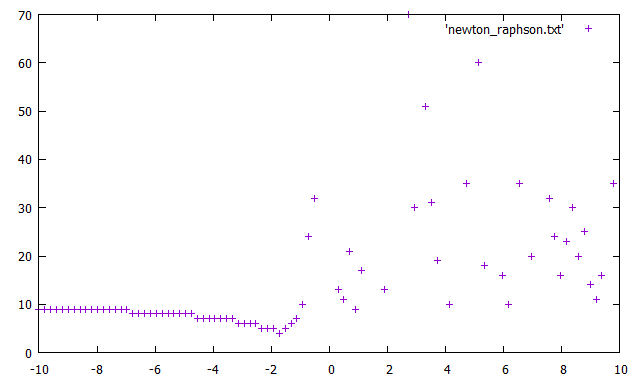
\includegraphics[scale = 0.6]{Figures/11_newton_raphson.png}
\end{figure}

A l'aide de la méthode \texttt{displayNoConvergence} on peut récupérer les $x_0$ pour lesquels Newton-Cotes ne converge pas. Voici la liste des points qui après 200 itérations n'ont pas trouvé de solution :

\begin{table}[H]
\centering
\begin{tabular}{|c|}
\hline
-0.30303030303030276\\
-0.10101010101010033\\
0.10101010101010033\\
1.3131313131313131\\
1.5151515151515156\\
1.7171717171717162\\
2.121212121212121\\
2.3232323232323235\\
2.525252525252524\\
3.1313131313131315\\
3.9393939393939394\\
4.3434343434343425\\
4.545454545454545\\
4.94949494949495\\
5.555555555555555\\
5.757575757575758\\
6.363636363636363\\
6.767676767676768\\
7.171717171717173\\
7.373737373737374\\
9.595959595959595\\
10.0\\
\hline
\end{tabular}
\end{table}
\subsubsection{Point 3}

On peut déduire du graphique qu'au plus $x_0$ est loin de la racine, au plus le nombre d'itérations nécessaires est élevé.

\subsection{Question 5}

\subsubsection{Point 1}

// TO DO

\subsubsection{Point 2}

// TO DO